\documentclass[francais]{beamer}
\usepackage[francais]{babel}
\usepackage[utf8]{inputenc}
\usepackage[T1]{fontenc}
\usepackage{lmodern}
\usepackage{amsmath, amssymb, amsfonts}




%CHOIX DU THEME et/ou DE SA COULEUR
% => essayer différents thèmes (en décommantant une des trois lignes suivantes)
%\usetheme{PaloAlto}
\usetheme{Madrid}

% => il est possible, pour un thème donné, de modifier seulement la couleur
\usecolortheme{default}
%\usecolortheme{whale}

%\useoutertheme[left]{sidebar}


%Pour le TITLEPAGE


\title[Nicolas Baillot d'Etivaux]{Constraining the equation of state for dense matter through thermal emission of neutron stars}


%Debut de la presentation :

\begin{document}


%Présentation:
\setbeamertemplate{blocks}[rounded]%
[shadow=false]


\begin{frame}{B matrix modeling}
 \begin{itemize}
  \item $L_b$: correlation lenght-scale, $var(\sigma^b)$.
  \item Grid point variance:\\
  $\sigma^b_i=1+var(\sigma^b)\times \sin(2\pi(i-1)/n), \quad i=1..n$
  \vspace{+0.5cm}
  \item Spectral variance:\\
  $\sigma^{b,spec}_0=1$\\
  $\sigma^{b,spec}_{2(i-1)}=2 \exp(-2(\pi(i-1)L_b)^2), \quad i=1..n/2$\\
  $\sigma^{b,spec}_{2(i-1)+1}=\sigma^{b,spec}_{2(i-1)}$\\
  $\sigma^{b,spec}_{n_{max}}=\exp(-2(\pi n_{max}/2)L_b)^2)$\\
 \end{itemize}
\end{frame}




\begin{frame}{Full resolution example}
\begin{center}
$\sigma^o$:0.01, n:128\\
 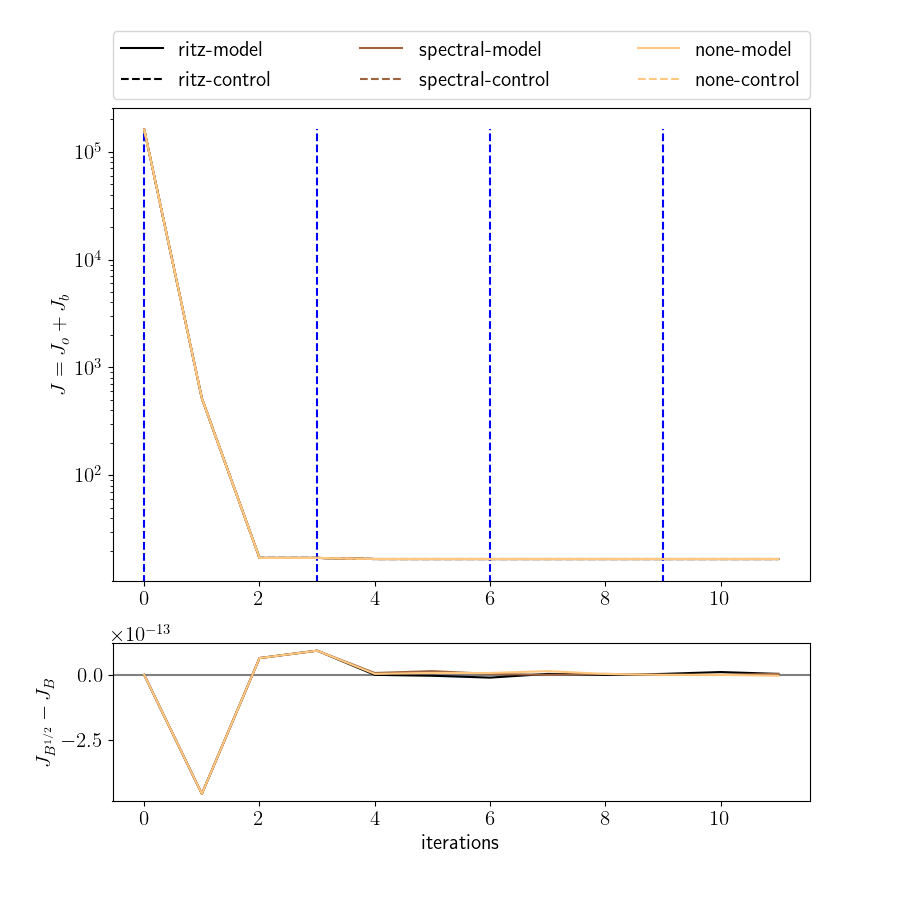
\includegraphics[scale=0.3]{./images/im1.png}
\end{center}
\end{frame}

\begin{frame}{Full resolution example with a more complex example}
\begin{center}
$\sigma^o$:0.1, n:2048\\
 \includegraphics[scale=0.3]{./images/im2.png}
\end{center}
\end{frame}


\begin{frame}{resolution x2}
\begin{center}
$\sigma^o$:0.01, n:128\\
 \includegraphics[scale=0.3]{./images/im3.png}
\end{center}
\end{frame}


\begin{frame}{resolution x2 - rho}
\begin{center}
$\sigma^o$:0.01, n:128\\
 \includegraphics[scale=0.3]{./images/im3_rho.png}
\end{center}
\end{frame}


\begin{frame}{resolution x2 - beta}
\begin{center}
$\sigma^o$:0.01, n:128\\
 \includegraphics[scale=0.3]{./images/im3_beta.png}
\end{center}
\end{frame}







\begin{frame}{resolution x1.5}
\begin{center}
$\sigma^o$:0.01, n:128\\
 \includegraphics[scale=0.3]{./images/im4.png}
\end{center}
\end{frame}


\begin{frame}{resolution x1.5}
\begin{center}
$\sigma^o$:0.01, n:128\\
 \includegraphics[scale=0.3]{./images/im4_rho.png}
\end{center}
\end{frame}





\begin{frame}{resolution x1.25}
\begin{center}
$\sigma^o$:0.01, n:128\\
 \includegraphics[scale=0.3]{./images/im5.png}
\end{center}
\end{frame}


\begin{frame}{resolution x1.25}
\begin{center}
$\sigma^o$:0.01, n:128\\
 \includegraphics[scale=0.3]{./images/im5_rho.png}
\end{center}
\end{frame}



\begin{frame}{resolution x2 - no spectral interpolation for grid points}
\begin{center}
$\sigma^o$:0.01, n:128\\
 \includegraphics[scale=0.3]{./images/im6.png}
\end{center}
\end{frame}



%BACKUP SLIDES:

\usebackgroundtemplate{}




\end{document}
